%!TEX root = main.tex


\subsection{Semantics of $\IFAMASS$} \label{subsect:semifamass}
% In this case, we only consider the intent flags.
%To define the semantics of $\IFAMASS$, we add some auxiliary functions and predicates. 


%To define the semantics of $\IFAMASS$, we adapt slightly the notion of configurations and the auxiliary functions and predicates. 

Recall that in an  $\STK$-dominating  $\IFAMASS$, $\lmd(A) = \STD$ and $\aft(A) = \aft(A_0)$ for each activity $A$. As a result, there is only one task in each configuration and the task allocation mechanism can be ignored here. Therefore, a configuration here is simply a word $[A_1,\cdots,A_m]\in\act^+$. 
% there is only one task in $\IFAMASS$.

%Before formally defining the semantics of $\Mm$, let us first describe the intuitions of the intent flags. 
%We would like to warn that although the intuitions of these intent flags may help the readers to get some preliminary idea of their meanings, before diving directly into the formal semantics, they are nonetheless inaccurate, especially when different flags may interfere with each other.

\paragraph{Intuitions}  We explain the intuitions of the five intent flags. 
\begin{itemize}
	\item $\stpflag$:  If it is set,  it has the same effect as starting an activity of the $\STP$ launch mode.
	\item $\ctpflag$:  If it is set, it will check for the existence of the started activity in the task. If the activity exists, then all the activities above the topmost occurrence of the started activity in the task will be removed. Otherwise, the started activity will be pushed into the task.
	\item $\rtfflag$:  If it is set, it will check for the existence of the started activity in the task. If the activity exists, then the topmost occurrence of this activity will be moved to the top of this task. Otherwise, the started activity will be pushed into the task.
	\item $\ntkflag$:  If it is set, it will look for an existing task to put the started activity according to the task allocation mechanism. If such a task exists, the task will be moved to the top and the started activity is pushed to the task, otherwise a new task is created to put this activity.
	\item $\ctkflag$: It is usually used together with $\ntkflag$. If it is set, it will remove all the activities in the task and push the started activity to the task.
\end{itemize}
%Moreover, $\ntkflag$ will only affect $\ctkflag$ in $\IFAMASS$, since there is only one task in $\IFAMASS$, task allocation mechanism will always allocate the top task.

%To define the semantics of $\IFAMASS$, the concept of configuration is adapted from the definition of configuration for $\LMAMASS$ as follows: A configuration of $\Mm$ is encoded as $[A_1,\cdots,A_m]\in\act^+$.

%Then we introduce some additional and adapted auxiliary functions and predicates that are to be used in the formal semantics of $\IFAMASS$.\\
We repeat the \textbf{Caveat} in Section~\ref{sect:semlmamass} for the intuition and introduce some additional functions and predicates. 
%\emph{Auxiliary functions and predicates.} 
For the configuration $\rho = [A_1,\cdots,A_m]$, 
%We define the following auxiliary functions and predicates.
\begin{itemize}
	% \item $\topact(\rho) = A_1$, $\btmact(\rho) = A_m$,
	%	\item $\push(\rho, B) = [B, A_1,\cdots,A_m]$,
	%	\item $\Pop(\rho) = [A_2,\cdots,A_m]$,
	% \item $\mvacttop(\rho, B) = ([B]\cdot S_1'\cdot S_1'', S_2, \cdots, S_n)$, if $S_1=S_1'\cdot[B]\cdot S_1''$ with $S_1'\in (\act\setminus\{B\})^*$,
	%	\item $\clrtop(\rho, B) = [A_j,\cdots,A_m]$, if $A_j = B$ for some $j\in[m]$ and $B\notin[A_1,\cdots,A_{j-1}]$,
	\item $\mvacttop(\rho, B) = [A_j,A_1,\cdots,A_{j-1},A_{j+1},\cdots A_m]$, if $A_j = B$ for some $j\in[m]$ and $B\notin[A_1,\cdots,A_{j-1}]$,
	\item $\clrtsk(\rho, B) = [B]$.
\end{itemize}

Intuitively $\mvacttop(\rho, B)$ is used for defining the semantics of $\rtfflag$, and $\clrtsk(\rho, B)$ is used for defining the semantics of $\ctkflag$.

%We are ready to define the semantics of $\IFAMASS$, that is, the relation $\rho \xrightarrow[\Mm]{\tau} \rho'$.
Let $\rho = [A_1,\cdots,A_m]$ for some $m\ge 1$ be the current configuration and $A_1 = A$. 

If $\tau = \back$ then $\rho' = \pop(\rho)$.

For the rule  $\tau = A\xrightarrow[]{\startactivity(\phi)}B$,

\begin{itemize}
	\item If $\phi\models\ctkflag\wedge\ntkflag$, then $\rho' = \clrtsk(\rho, B)$.
	\item Otherwise,
	\begin{itemize}
		\item if $\phi \models\ctpflag$ and $B \in \rho$, then $\rho' =\clrtop(\rho, B)$,
		\item otherwise,
		\begin{itemize}
			\item if $\phi \models \rtfflag$ and $B \in \rho$, then $\rho'=\mvacttop(\rho, B)$,
			\item otherwise,
			\begin{itemize}
				\item if $\phi \models \stpflag$ and $A = B$, then $\rho' = \rho$,
				\item otherwise, $\rho' = \push(\rho, B)$.
			\end{itemize}
		\end{itemize}
	\end{itemize}
\end{itemize}

We use the following example to illustrate the semantics.
\begin{example}
	Let $\Mm = (\act,A,\lmd,\aft,\Delta)$ be an $\IFAMASS$, where $\act = \{A,B,C,D\}$, where for each $A'\in\act$, $\lmd(A') = \STD$ and $\aft(A') = 1$. 
	Moreover, $\Delta = \{\back,\tau_1, \tau_2, \tau_3, \tau_4, \tau_5, \tau_6\}$, where 
	% $\rho_0 = (([D_1],D_1,1))$, and\
	$\tau_1 = A \xrightarrow{\startactivity(\ctkflag)} B$,
	$\tau_2 = B \xrightarrow{\startactivity(\rtfflag)} C$,
	$\tau_3 = C \xrightarrow{\startactivity(\ctpflag)} B$,
	$\tau_4 = C \xrightarrow{\startactivity(\rtfflag)} B$,
	$\tau_5 = C \xrightarrow{\startactivity(\ntkflag\wedge\ctkflag)} D$,
	$\tau_6 = D \xrightarrow{\startactivity(\stpflag)} D$.
	Then the configurations that are reachable from the initial configuration $[A]$ by executing the transition rules from $\Delta$ are illustrated in Figure~\ref{ifasm-example}, where the vertices denote the configurations and the edges denote the elements of $\xrightarrow[\Mm]{}$. 
	For instance, 
	\begin{itemize}
		\item if $A \xrightarrow{\startactivity(\ctkflag)} B$ is applied to the configuration $[A]$, then $B$ is pushed, since $\phi\models\neg\ntkflag \wedge \neg \ctpflag \wedge \neg \rtfflag \wedge \neg \stpflag$, resulting in the configuration $[BA]$,
		%
		\item if $B \xrightarrow{\startactivity(\rtfflag)} C$ is applied to the configuration $[BA]$, then $C$ is pushed, since $\phi\models\rtfflag$ and $C$ does not occur in the task $[BA]$, resulting in the configuration $[CBA]$,
		%
		\item if $C \xrightarrow{\startactivity(\ctpflag)} B$ is applied to the configuration $[CBA]$, then all the activities above $B$, which is $C$ here, are removed from the task, since $\phi\models\ctpflag$ and $B$ occurs in the task $[CBA]$, resulting in the configuration $[BA]$,
		%
		\item if $C \xrightarrow{\startactivity(\rtfflag)} B$ is applied to the configuration $[CBA]$, then $B$ is moved to the top of the task, since $\phi\models\rtfflag$ and $B$ occurs in the task $[CBA]$, resulting in the configuration $[BCA]$,
		%
		\item if $B \xrightarrow{\startactivity(\rtfflag)} C$ is applied to the configuration $[BCA]$, then $C$ is moved to the top of the task, since $\phi\models\rtfflag$ and $C$ occurs in the task $[BCA]$, resulting in the configuration $[CBA]$,
		%
		\item if $C \xrightarrow{\startactivity(\ntkflag\wedge\ctkflag)} D$ is applied to the configuration $[CBA]$, then all activities are removed from the task and $D$ is pushed, since $\phi\models\ntkflag\wedge\ctkflag$, resulting in the configuration $[D]$,
		%
		\item if $D \xrightarrow{\startactivity(\stpflag)} D$ is applied to the configuration $[D]$, then $D$ is not pushed, since $\phi\models\stpflag$ and $D$ is the top activity of the task, resulting to the configuration $[D]$.
	\end{itemize}
	Note that for $\Mm$, there are only finitely many configurations reachable from the initial configuration, which may not be the case for $\IFAMASS$ in general.  
	% $(([D_1],D_1,1))$\\
	% $\xrightarrow[\tau_1]{\Mm}(([P_1D_1],D_1,1))$\\
	% $\xrightarrow[\tau_2]{\Mm}(([P_1D_1],D_1,1))$\\
	% $\xrightarrow[\tau_3]{\Mm}(([K_2],K_2,0),([P_1D_1],D_1,1))$\\
	% $\xrightarrow[\tau_4]{\Mm}(([D_1K_2],K_2,0),([P_1D_1],D_1,1))$\\
	% $\xrightarrow[\tau_5]{\Mm}(([T_2],T_2,0),([D_1K_2],K_2,0),([P_1D_1],D_1,1))$\\
	% $\xrightarrow[\tau_6]{\Mm}(([K_2],K_2,0),([T_2],T_2,0),([P_1D_1],D_1,1))$\\
	
	
	
	\begin{figure}
		% \vspace{-3mm}
		\centering
		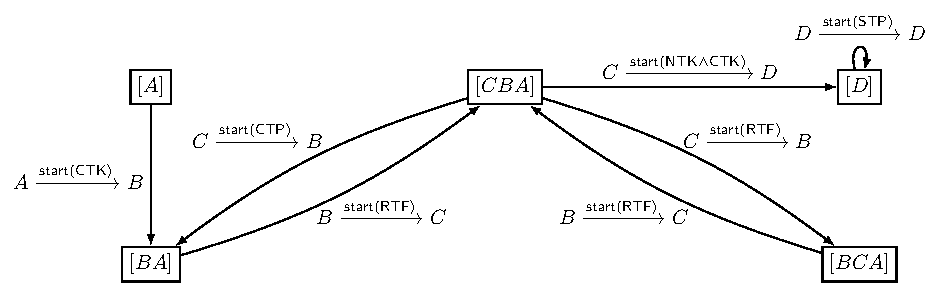
\includegraphics[scale = 0.8]{ifasm-example.pdf}
		\caption{Configurations reachable from the initial configuration $[A]$ in an $\IFAMASS$ $\Mm$}
		%in $\phi$
		% \vspace{-6mm}	
		\label{ifasm-example}
	\end{figure}
\end{example}
% In this case, we assume that the launch modes of activities are $\STD$.  Intuitively, for a transition $A\xrightarrow{\startactivity(\phi)}B$, the intent flags in $\phi$ may depend on each other. The dependency can exhibit in the following two forms: (1) $n$ \emph{subsumes} $n'$, i.e., $n'$ is ignored if $n$ co-occurs with $n'$, and the ``subsume'' relations are transitive, (2) $n$ \emph{enables} $n'$, i.e., $n'$ takes effect if $n$ co-occurs with $n'$. We summarize the dependencies among the intent flags in Figure xxx, 

% For a transition $A\xrightarrow{\startactivity(\phi)}B$, we conclude that :
% \begin{itemize}
	% 	\item when $\ctkflag$ tasks effect, then the task will be cleared, and $B$ is pushed into the task,
	% 	\item when $\ctpflag$ tasks effect, then the task will be poped until the top activity is $B$ when $B$ is in the task, $B$ will be pushed into the task otherwise, which is similar with the case $\lmd(B) = \STK$,
	% 	\item when $\rtfflag$ tasks effect, then $B$ is escalated to the top of the task when $B$ is in the task, $B$ will be pushed into the task otherwise, 
	% 	\item when $\stpflag$ tasks effect, then $B$ is pushed into the task when the top activity of the task is not $B$, which is similar with the case $\lmd(B) = \STP$.
	% \end{itemize}

